\chapter{Paralelización en GPU de algorítmos de búsqueda de caminos óptimos.}
\chapterauthor{Diego De Pablo}
\section{Resumen}
Este trabajo explora la viabilidad de la paralelización para la búsqueda de caminos óptimos en grafos, utilizando como caso de estudio el algoritmo de Dijkstra. El objetivo principal es evaluar la eficiencia de una implementación paralela en Java comparandola con su versión secuencial original, centrándose en el análisis del tiempo de ejecución y la precisión de los resultados.

La recurrencia, inherente a la naturaleza de los grafos, presenta un desafío computacional significativo al tratar con problemas de gran escala. La paralelización en GPU emerge como una alternativa prometedora para abordar este reto, aprovechando la arquitectura altamente paralela de las GPU para acelerar el proceso de búsqueda de caminos. Si bien en este trabajo se centrará tanto en la parte teórica como la implementación de lo visto, la amplitud y complejidad del tema han hecho necesario enfocarse en el algoritmo de Dijkstra, dejando otros aspectos para futuras investigaciones.

Los resultados obtenidos revelaron que la implementación paralela en Java ofrece mejoras significativas en el tiempo de ejecución al hablar de grafos grafos completos o con un número elevado de nodos. En el caso de grafos con menor densidad o complejidad, la implementación paralela no mostró una ventaja significativa sobre la versión secuencial. No obstante, los resultados generales confirman el potencial de la paralelización para optimizar la búsqueda de caminos óptimos en grafos.

En esencia, la paralelización en grafos consiste en dividir el grafo original en subgrafos más pequeños y manejables. Esto permite distribuir la carga computacional entre múltiples procesadores, lo que puede traducirse en una reducción significativa del tiempo de ejecución, especialmente para problemas de gran escala.

\textbf{Palabras clave:} Paralelismo, Dijkstra, Búsqueda de caminos más cortos, Grafo, Java, GPU. 

\section{Introducción}

Los grafos, estructuras matemáticas que representan relaciones entre entidades, han trascendido su rol tradicional en las matemáticas para convertirse en un lenguaje universal capaz de modelar y analizar sistemas complejos en una amplia gama de disciplinas. Desde la logística y la planificación de rutas hasta la optimización de diversas ramas de la bioinformática, su versatilidad los convierte en una herramienta invaluable para abordar problemas desafiantes en la era de la información. 

En el ámbito de la optimización, una de las tareas más relevantes es la búsqueda de caminos óptimos entre pares de nodos en un grafo. Estos caminos, que representan las rutas más eficientes para conectar dos puntos,  la literatura científica ofrece diversos algoritmos para la búsqueda de caminos óptimos en grafos. Entre los más conocidos se encuentran los algoritmos de Dijkstra, a* (Estrella), Floyd y Dantzig, descritos y comparados por \cite{Minieka}. Estos algoritmos proporcionan soluciones eficientes para encontrar los caminos más cortos entre pares de nodos, lo que los convierte en herramientas valiosas para resolver problemas de optimización en diversos campos.

A pesar de ello, como indica \cite{Harish}, la aplicación de estos algoritmos secuenciales sobre grafos de gran tamaño presenta un reto computacional significativo. La complejidad computacional de estos algoritmos crece exponencialmente con el número de nodos y aristas del grafo, lo que puede traducirse en tiempos de ejecución prohibitivamente largos para problemas de gran escala.
En este contexto, la computación paralela surge como una alternativa prometedora para abordar este desafío. La computación paralela, que distribuye la carga computacional entre múltiples procesadores, permite obtener mejoras significativas en el rendimiento de algoritmos computacionalmente intensivos, como los algoritmos de búsqueda de caminos óptimos en grafos.

Las Unidades de Procesamiento Gráfico (GPU), inicialmente concebidas para la rápida generación de imágenes en gráficos 3D, han experimentado una notable evolución, transformándose en coprocesadores altamente paralelos con un enorme potencial para la computación general. A diferencia de los procesadores centrales tradicionales (CPU), las GPU poseen una arquitectura altamente paralela que les permite ejecutar múltiples tareas de forma simultánea. Esta característica las convierte en herramientas ideales para acelerar algoritmos que se benefician de la paralelización, como los de búsqueda de caminos óptimos en grafos. 
 Tal como lo expresa \cite{Boyer} demostraron que el uso de GPU para la búsqueda de caminos óptimos en grafos puede proporcionar mejoras significativas de rendimiento en comparación con las implementaciones secuenciales en CPU. Esta capacidad de aceleración se debe a la arquitectura paralela de las GPU, que permite distribuir la carga computacional entre miles de núcleos de procesamiento, lo que reduce significativamente el tiempo de ejecución de los algoritmos.

Al igual que otros capítulos de este libro, este se centra en evaluar la eficacia de la paralelización en un área específica de estudio: la búsqueda de caminos óptimos. Para ello, analizaremos en profundidad el algoritmo de Dijkstra y otros algoritmos de búsqueda de caminos óptimos, explorando las posibilidades de paralelización en cada uno de ellos.

Nuestro objetivo no solo es evaluar la viabilidad de la paralelización en este campo, sino también servir de inspiración y contribuir al avance de la comprensión de esta técnica en el contexto de la computación con GPU y el uso de grafos. Aspiramos a proporcionar información valiosa que impulse el desarrollo de nuevas técnicas de optimización más eficientes y escalables.

\section{Tema de Estudio}

Según el autor \cite{Wilson}), al modelar un sistema como un grafo, las entidades que lo componen se representan como nodos y las relaciones entre estas entidades se representan como arcos que conectan los nodos. Esta representación gráfica permite analizar las propiedades del sistema de manera eficiente y estudiar las interacciones entre sus componentes.

Una forma de emplear los grafos son los algoritmos de búsqueda de caminos más cortos entre pares de nodos. Estos algoritmos son capaces de identificar la ruta más eficiente para conectar dos puntos en un grafo. El significado de "camino óptimo" puede variar según el sistema que se modele. Para una comerciante, por ejemplo, \cite{Minieka} señala que este camino se traduce como el conjunto de transacciones que genera el mayor beneficio económico. En caso de ser un vendedor ambulante, se convierte en la ruta de ventas que maximiza sus ganancias. Y para una aerolínea es el camino que se traduce en la ruta de vuelo que minimiza el tiempo en el aire.

En el vasto universo de la teoría de grafos, el algoritmo de Dijkstra se erige como un faro que guía a través del complejo laberinto de nodos y arcos, iluminando el camino más corto entre dos puntos. Esta herramienta matemática, desarrollada por el informático holandés Edsger Dijkstra en 1956, se ha convertido en un pilar fundamental para la resolución de problemas de búsqueda y optimización en diversos campos.

El algoritmo de Dijkstra, también conocido como algoritmo de etiquetas, \cite{free} explica como el algoritmo opera de manera sistemática, explorando el grafo paso a paso. Comienza seleccionando un nodo inicial (punto de partida) y lo marca como visitado. A continuación, calcula la distancia más corta entre el nodo actual y cada uno de los nodos no visitados, utilizando una función de peso asignada a cada arco.
El nodo no visitado con la distancia más corta se convierte en el nuevo nodo actual, y el proceso se repite. Se actualizan las distancias de los nodos no visitados adyacentes al nuevo nodo actual, tomando en cuenta la distancia mínima encontrada hasta el momento. Esta exploración continua hasta que se alcanza el nodo final (punto de destino).

En este trabajo se desea abordar temas aunque sea de manera superficial que estan estrechamente relacionados con la paralelización de algorítmos de búsqueda de caminos óptimos, si bien cada algoritmo abarca tema suficiente para una tesís, en este trabajo se plantea iniciar el camino aunque sea de manera teorica de otros algoritmos además del Dijkstra para una futura implementación paralela, se mencionarán  Floyd, Dantzig y A* (estrella), entre otros. Además de considerarse las distintas herramientas para paralelizar como podría ser el concepto de procesamiento por lotes, paralelizar el propio algoritmo, entre otros. 

\section{Objetivo}

\begin{itemize}
  \item Evaluar la eficiencia de la paralelización de los algoritmos de búsqueda de caminos más cortos entre los nodos de un grafo, comparando su versión secuencial con su versión paralela.
  \item Considerar teóricamente las herramientas capaces de paralelizar un algoritmo de búsqueda de caminos más cortos, buscando el mejor método en cuanto a facilidad de implementación, reutilización y resultados.
  \item Comparar tiempos de ejecución y exactitud de los resultados para el algoritmo de Dijkstra en su implementación secuencial y paralela.
\end{itemize}

\section{marco teórico}

La concurrencia, en el ámbito de la computación, se asemeja a una coreografía precisa donde múltiples procesos comparten el escenario del procesador, ejecutando sus pasos de manera simultánea. A diferencia de la ejecución secuencial, donde cada proceso espera su turno pacientemente, la concurrencia permite que los procesos avancen en paralelo, aprovechando al máximo los recursos disponibles. Como resume \cite{oscar} cada núcleo representa un espacio independiente donde un proceso puede desplegar su coreografía. De esta manera, un procesador con cuatro núcleos puede albergar hasta cuatro procesos ejecutando sus instrucciones de forma simultánea, como si se tratara de cuatro bailarines independientes en un mismo escenario.

No obstante, la concurrencia no implica que todos los procesos reciban la misma atención del procesador de manera uniforme. La planificación del sistema operativo determina el orden en que los procesos acceden a los recursos compartidos, como la memoria y la unidad central de procesamiento. Es decir, los procesos comparten el escenario, pero no necesariamente al mismo tiempo.

Como sigue explicando \cite{oscar} el paralelismo, en el ámbito de la computación, adopta la filosofía de "divide y vencerás" para abordar problemas complejos de manera más eficiente. En lugar de tratar un problema como una entidad única, el paralelismo lo descompone en subproblemas más pequeños y manejables, asignando cada uno a un procesador o unidad de procesamiento independiente.

Podrías extrapolarse en un ejemplo de un rompecabezas gigante. En un enfoque secuencial, se tendría que armar cada pieza una a una, lo que podría llevar mucho tiempo. Sin embargo, el paralelismo nos permite dividir el rompecabezas en secciones más pequeñas, enfoca elementos de poco nivel y esfuerzo en unir una porción de las piezas. Una vez que cada elemento ha completado su sección, al unir todas las soluciones coincidirá con la solución final de manera mucho más rápida.

La clave del paralelismo reside en la descomposición efectiva del problema en subproblemas independientes. Si la descomposición no es adecuada, la comunicación entre las unidades de procesamiento puede convertirse en un cuello de botella, ralentizando el proceso general.

\begin{figure}[h]
	\centering 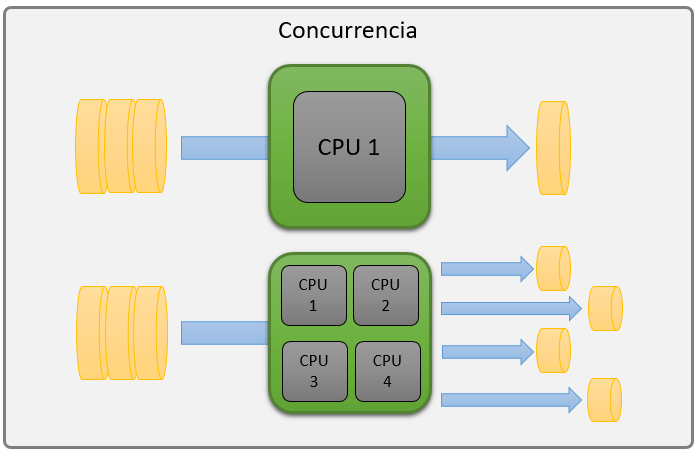
\includegraphics[width=0.65\linewidth]{img/Concurrencia_1.png}
	\caption{Secuencial contra Paralelo by Oscar Blancarte}
	\label{fig:etiqueta1}
\end{figure}

 La posibilidad de dividir un problema en tareas más pequeñas que se ejecutan simultáneamente, conocida como paralelismo, abre la puerta a un significativo aumento en el rendimiento computacional. Esto resulta especialmente ventajoso cuando se trabaja con equipos que cuentan con múltiples procesadores \cite{Stallings}

Una vez conocido el concepto de paralelismo, el siguiente tópico que se debe resaltar son los grafos, es el problema principal que se plantea en este capitulo. En el libro "Introduction to Graph Theory" \cite{Wilson} se introduce al concepto de grafos como una poderosa herramienta para modelar y analizar sistemas complejos. Estos entes matemáticos, compuestos por nodos (entidades del sistema) y arcos (relaciones entre entidades), nos permiten representar una amplia gama de escenarios, desde redes de transporte y comunicación hasta estructuras moleculares y relaciones sociales.

Según \cite{Wilson}, la versatilidad de los grafos radica en su capacidad para capturar la esencia de un sistema, abstraer sus elementos fundamentales y revelar las interacciones que los definen. Un mismo grafo puede representar diversas realidades: una red eléctrica (Figura 2.2), un mapa de caminos con nodos como ciudades y aristas como caminos (Figura 2.3), entre muchas otras, estos escenarios pueden ser representados en un grafo aún más simple en el que trabajar comodamente(Figura 2.4).

\begin{figure}[h]
	\centering 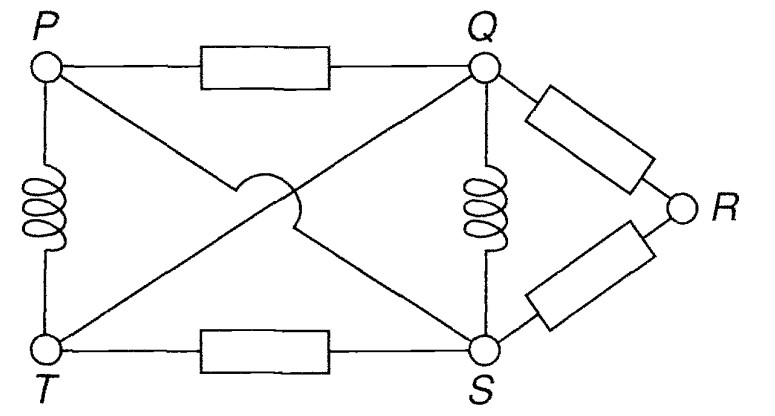
\includegraphics[width=0.45\linewidth]{img/red_electrica_expresada_como_grafo2.jpg}
	\caption{Secuencial contra Paralelo by Robin J. Wilson }
	\label{fig:etiqueta1}
\end{figure}

\begin{figure}[h]
	\centering 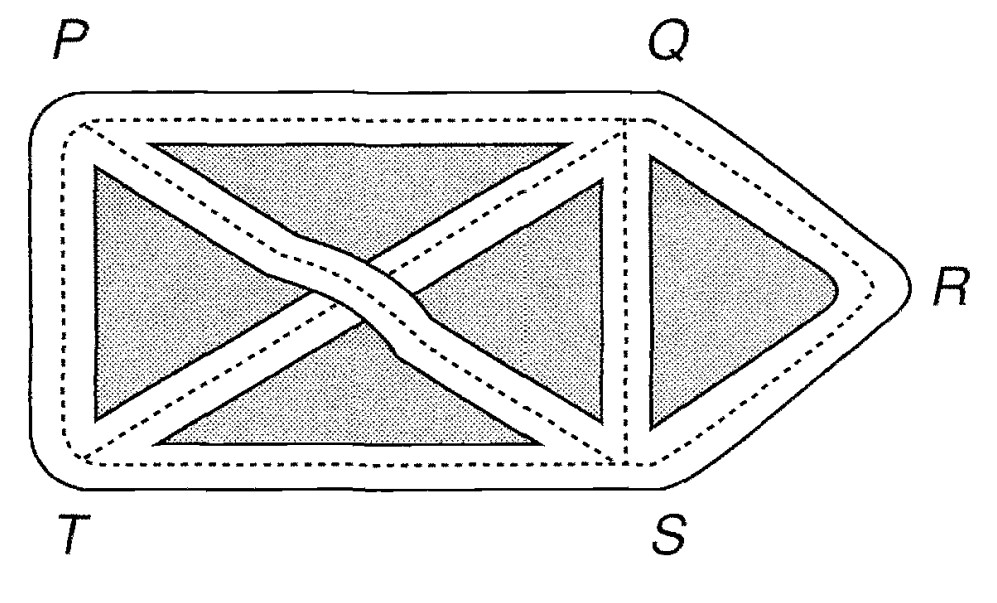
\includegraphics[width=0.45\linewidth]{img/caminos_expresado_como_grafo3.jpg}
	\caption{Mapa de caminos by Robin J. Wilson}
	\label{fig:etiqueta1}
\end{figure}

\begin{figure}[h]
	\centering 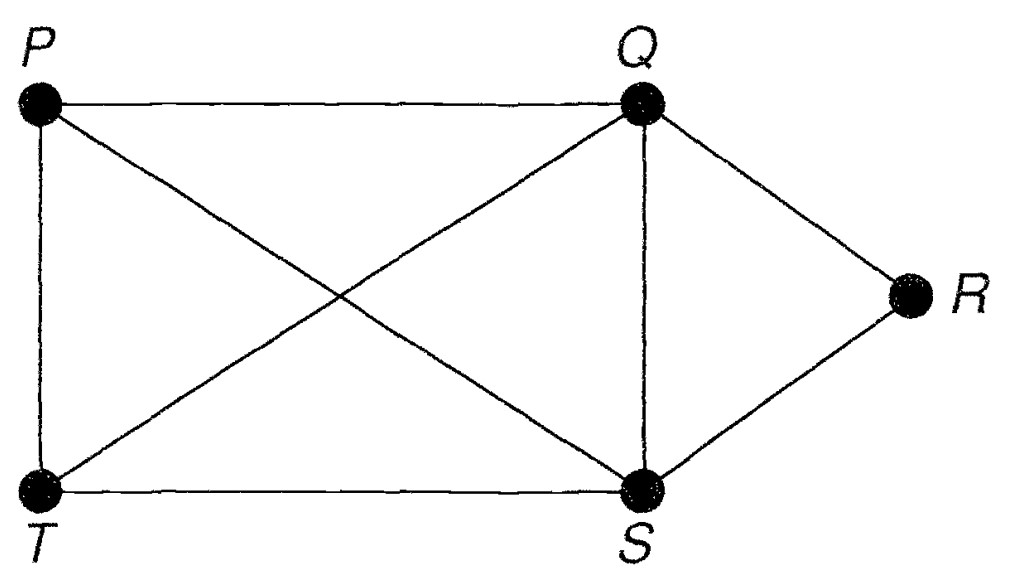
\includegraphics[width=0.45\linewidth]{img/grafo_simplificado4.jpg}
	\caption{grafo simplificicado by Robin J. Wilson}
	\label{fig:etiqueta1}
\end{figure}

En el vasto universo de la teoría de grafos, los algoritmos de búsqueda de caminos más cortos se erigen como brújulas infalibles para navegar por el laberinto de nodos y arcos. Estos algoritmos, como su nombre lo indica, tienen como objetivo encontrar la secuencia de arcos que conecta dos nodos en un grafo, minimizando el costo total del recorrido.

En palabras de \cite{deo}, la búsqueda de caminos más cortos trasciende su propósito original y se convierte en el equivalente matemático de una amplia gama de problemas de optimización. La naturaleza del grafo que se modela otorga a estas rutas óptimas un significado específico, haciéndolas útiles en diversos contextos.

La versatilidad de estos algoritmos radica en su capacidad para adaptarse a diversos escenarios y problemáticas. Desde redes de transporte y comunicación hasta sistemas de distribución y logística, la búsqueda de caminos más cortos se convierte en una herramienta indispensable para la toma de decisiones óptimas.

\begin{figure}[h]
	\centering 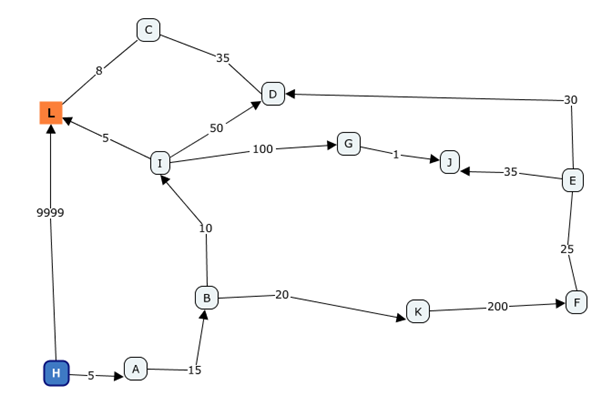
\includegraphics[width=0.58\linewidth]{img/Grafo_ejemplo_5.png}
	\caption{Ejemplo de un grafo ponderado no dirigido by Diego De Pablo (Elaboración propia)}
	\label{fig:etiqueta1}
\end{figure}

El algoritmo de Dijkstra se utiliza para encontrar el camino más corto entre un nodo inicial A a un nodo final B. Para ello evalúa las distancias conocidas desde el nodo s a los otros nodos, empezando por aquellos con la menor distancia y actualizando la información cada vez que se evalúa un nuevo nodo. De esta forma se recorre el grafo hasta hallar la menor distancia al nodo t. A continuación se detalla el funcionamiento del algoritmo, conforme a la explicación de \cite{Minieka}. A continuación se ejemplifica su ejecución, en la figura 2.5 se observa un grafo ponderado cuyo nodo inicial es H y nodo final es L:

\subsection*{Paso 1: Inicialización}
Se marcan todos los nodos como no visitados y se asigna una distancia inicial de $d(s) = 0$ al nodo origen $s$, y $d(x) = \infty$ para todos los demás nodos $x \neq s$. El nodo $s$ se marca como visitado y se almacena en la variable $y$.

\subsection*{Paso 2: Actualización de distancias}
Para cada nodo no visitado $x$, se actualiza $d(x)$ como el mínimo entre su distancia actual y la suma de $d(y)$ más el peso del arco $(y, x)$, si existe. Si no hay arco, la distancia permanece infinita.

\subsection*{Paso 3: Condición de parada}
Si $d(x) = \infty$ para todos los nodos no visitados, el algoritmo termina, indicando que no hay más caminos accesibles desde el nodo origen.

\subsection*{Paso 4: Iteración}
Se selecciona el nodo no visitado $x$ con la menor distancia $d(x)$, se marca como visitado, y se actualiza $y$ con el nodo $x$ para la próxima iteración.

\subsection*{Paso 5: Comprobación del nodo destino}
Si el nodo destino $t$ ha sido visitado, el algoritmo finaliza, habiendo encontrado el camino más corto de $s$ a $t$.

\subsection*{Paso 6: Repetición}
Si el nodo destino $t$ no ha sido visitado, se vuelve al Paso 2 hasta que se cumpla la condición de parada o se encuentre el camino al nodo destino.

\begin{figure}[h]
	\centering 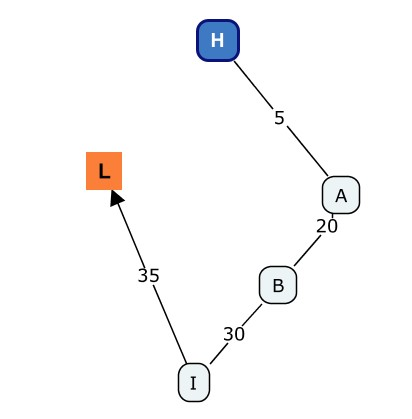
\includegraphics[width=0.38\linewidth]{img/Solucion_final_6.jpg}
	\caption{Ejemplo de camino óptimo by Diego De Pablo (Elaboración propia)}
	\label{fig:etiqueta1}
\end{figure}

\cite{deo} propone una interpretación del algoritmo de Dijkstra en la que el grafo se representa como una matriz D = [dij], donde dij representa la distancia entre el nodo i y el nodo j. Esta matriz simplifica la programación del algoritmo, pero los pasos y el funcionamiento subyacente siguen siendo los mismos.

\cite{Minieka} señala que el algoritmo de Dijkstra en su forma original no funciona correctamente si el grafo contiene arcos con pesos negativos. Esto se debe a que al marcar un nodo, este nunca se vuelve a evaluar, lo que puede llevar a resultados erróneos. Existen modificaciones al algoritmo para manejar este tipo de casos, pero no se profundizarán en este trabajo.

Un termino importante a destacar es la relajación de aristas es un concepto fundamental en el algoritmo de Dijkstra para encontrar el camino más corto entre dos nodos en un grafo. \cite{Cormen} Explica como esta técnica se basa en la actualización iterativa de las distancias estimadas a cada nodo, tomando en cuenta los pesos de las aristas y las distancias ya calculadas.

Formalmente para , la relajación de una arista $(u,v)$ implica comparar la distancia actual estimada a $v$ (denotada como $d_v$) con la suma de la distancia estimada actual a $u$ (denotada como $d_u$) y el peso de la arista $(u,v)$, representado por $w_{uv}$. Si esta suma es menor que $d_v$, se actualiza el valor de $d_v$ a la nueva distancia estimada.

En otras palabras, la relajación de una arista verifica si existe un camino más corto a un nodo a través de la arista en cuestión. Si se encuentra un camino más corto, se actualiza la distancia estimada al nodo para reflejar esta nueva información.

La relajación de aristas se repite iterativamente hasta que se hayan considerado todas las aristas del grafo. Una vez finalizado el proceso, las distancias estimadas almacenadas en cada nodo representan las distancias más cortas reales entre el nodo origen y todos los demás nodos del grafo.

Esta técnica es crucial para el funcionamiento eficiente del algoritmo de Dijkstra, ya que permite identificar y actualizar de manera incremental los caminos más cortos a medida que se exploran las aristas del grafo.


\cite{deo} analiza la complejidad temporal del algoritmo de Dijkstra, concluyendo que el tiempo de ejecución es independiente de la cantidad de arcos en el grafo. Esto se debe a que, implícitamente, se asume que los arcos inexistentes sí existen, pero con pesos muy altos. El mismo autor demuestra que el tiempo de ejecución es proporcional a \( n^2 \), donde n es el número de nodos en el grafo.

A continuación una listas de algoritmos similares que podremos paralelizar de manera muy similar al algoritmo de dijkstra.

\begin{itemize}
  \item El algoritmo de Floyd tiene como objetivo encontrar los caminos más cortos entre todos los pares de nodos en un grafo. Es considerado uno de los algoritmos más eficientes para esta tarea, junto con el algoritmo de Dantzig, según \cite{Dreyfus}. Su tiempo de ejecución es proporcional a \( n^3 \), donde n es el número de nodos en el grafo, como indica \cite{deo}.
  \item El algoritmo de Dantzig, al igual que el algoritmo de Floyd, busca encontrar los caminos más cortos entre todos los pares de nodos en un grafo. Conforme \cite{Minieka}, ambos algoritmos realizan los mismos cálculos, pero en un orden diferente. \cite{deo} indica que su tiempo de ejecución es proporcional a \( n^3 \) y su eficiencia es comparable al algoritmo de Floyd. 
  \item El algoritmo A* (estrella) muy parecido al algoritmo de Dijkstra con la diferencia de aplicar una función heurística, \cite{Dreyfus} lo define como un algoritmo de búsqueda heurística que busca el camino más corto entre un nodo origen y un nodo destino en un grafo. A diferencia de otros algoritmos de búsqueda como la búsqueda en anchura o en profundidad, A* utiliza una función heurística para estimar la distancia restante al nodo destino, lo que le permite enfocarse en los caminos más prometedores y mejorar su eficiencia.
\end{itemize}

Ya conociendose los conceptos de paralelismo, grafos y sus algoritmos, es importante destacar que los algoritmos tradicionales suelen estar diseñados para una ejecución secuencial, donde las operaciones se realizan una tras otra. Como dicta \cite{Stallings} para aprovechar las ventajas del paralelismo, es necesario rediseñarlos y adaptarlos, dividiéndolos en fracciones de trabajo independientes que puedan ejecutarse en paralelo sin generar conflictos.

A mayor paralelismo, es decir, a mayor cantidad de tareas que se ejecutan simultáneamente, mayor será la reducción en el tiempo de ejecución total. Pese a todo, es importante considerar que la ejecución paralela requiere de hardware compatible.

Independientemente de la cantidad de subtareas en que se divida un programa, solo podrán ejecutarse en paralelo la cantidad que permita el procesador o los procesadores del equipo. Por lo tanto, el costo del hardware también debe ser un factor a considerar en el diseño de soluciones.

Las Unidades de Procesamiento Gráfico (GPU), originalmente diseñadas para la generación rápida de imágenes para su visualización en pantalla, han demostrado ser altamente paralelas y útiles para la decodificación de vídeo y la creación de gráficos 3D \cite{Randima}.

De todas formas, su potencial no se limita a estas áreas, ya que también pueden ser empleadas para resolver problemas en otros ámbitos, dando lugar a lo que se conoce como Programación de Propósito General en Unidades de Procesamiento Gráfico (GPGPU).

Como establece \cite{Cormen} el algoritmo de Dijkstra, por su naturaleza secuencial, presenta un desafío a la hora de paralelizarlo. Pero no es imposible, existen diversas estrategias que pueden ser empleadas para mejorar su rendimiento en arquitecturas con múltiples procesadores, entre ella destaca la partición de grafo y paralelización del cálculo dentro de un subgrafo. 

En cuanto a la partición de grafo, dividir el grafo original en subgrafos más pequeños y manejables.Asignar el cálculo de las rutas más cortas dentro de cada subgrafo a un procesador diferente. Combinar los resultados parciales obtenidos de cada subgrafo para determinar las rutas más cortas entre todos los pares de nodos del grafo original.

Por parte de la paralelización del cálculo dentro de un subgrafo, en un subgrafo específico, paralelizar el cálculo de las distancias mínimas desde un nodo origen a todos los demás nodos del subgrafo. Esto puede implicar la exploración simultánea de múltiples rutas potenciales desde el nodo origen. Se pueden emplear algoritmos paralelos como BFS (Búsqueda en anchura) o DFS (Búsqueda en profundidad) modificados para aprovechar el paralelismo.

Esta última fue evaluada por \cite{Luo} Los autores proponen un algoritmo de Dijkstra paralelo que aprovecha la arquitectura altamente paralela de las GPUs. El algoritmo divide el cálculo de las rutas más cortas en tareas independientes que pueden ejecutarse simultáneamente en los múltiples núcleos de la GPU. Esto permite un procesamiento más rápido en comparación con el algoritmo de Dijkstra secuencial.

El artículo describe la implementación del algoritmo en CUDA, un lenguaje de programación paralelo para GPUs de NVIDIA. Además, los autores evalúan el rendimiento del algoritmo propuesto en diferentes escenarios y comparan su desempeño con el algoritmo de Dijkstra secuencial. Los resultados demuestran que el algoritmo paralelo de Dijkstra basado en GPU puede lograr mejoras significativas en la velocidad de cálculo, especialmente para grafos de gran tamaño.

Otra investigación interesante nace del grupo \cite{Crauser} El artículo titulado en español "Paralelización del algoritmo de camino más corto de Dijkstra" se centra en la paralelización del algoritmo de Dijkstra. El algoritmo original de Dijkstra es secuencial, Como ya se mencionó esto puede ser ineficiente en arquitecturas con múltiples procesadores.

Los autores del artículo proponen un algoritmo PRAM (Parallel Random Access Machine) para paralelizar el algoritmo de Dijkstra. El algoritmo PRAM divide el trabajo en fases que pueden ejecutarse en paralelo. Los autores analizan el rendimiento del algoritmo PRAM y muestran que puede mejorar significativamente el rendimiento del algoritmo de Dijkstra original en arquitecturas con múltiples procesadores.

El algoritmo PRAM (Parallel Random Access Machine) es un modelo de computación teórico que describe una máquina paralela con acceso aleatorio a una memoria compartida. Se utiliza para analizar la complejidad paralela de algoritmos y evaluar su eficiencia en arquitecturas con múltiples procesadores.

El artículo también presenta extensiones del algoritmo PRAM para computación en memoria externa. Esto es útil para grafos grandes que no caben en la memoria principal. Las simulaciones muestran que el enfoque propuesto es aplicable incluso en grafos no aleatorios.


\section{Resultados y análisis de código}

Tras revisar las herramientas teóricas para paralelizar el algoritmo de búsqueda de caminos más cortos, se ha observado que el algoritmo de Dijkstra, diseñado originalmente para un procesamiento secuencial, ha sido objeto de diversas modificaciones para su paralelización. Entre estas soluciones se encuentran el uso de múltiples hebras para aumentar la velocidad de cálculo y la división del grafo en subgrafos.

Sin embargo, en este trabajo se propone un enfoque alternativo que centra el paralelismo en la creación de tareas concurrentes para relajar las aristas de los nodos vecinos. Esta estrategia permite procesar simultáneamente múltiples aristas, aprovechando los múltiples núcleos de la CPU para acelerar la ejecución.

Para demostrar la utilidad de la paralelización en este contexto, en lugar de aplicar el algoritmo una sola vez buscando un nodo origen y un nodo destino, se planteará una tarea más compleja: la búsqueda de todos los caminos óptimos que parten del nodo origen hacia todos los demás nodos del grafo. De esta manera, se pondrá a prueba la capacidad del algoritmo paralelo para manejar una tarea computacionalmente más exigente.

Antes de comparar el rendimiento de las versiones secuencial y paralela del algoritmo de Dijkstra, es crucial verificar el correcto funcionamiento de ambas implementaciones. Para ello, se desarrollarán dos versiones del algoritmo: una secuencial y otra paralela. Ambas versiones estarán diseñadas para resolver el problema de búsqueda de caminos óptimos en el grafo presentado en la Figura 2.5, tomando como nodo inicial el nodo H y considerando todos los nodos restantes como destinos.

El código implementado aparecerá detalladamente en el apartado de apéndice, pero haré un breve resumen de cada código, en el caso del código 1, es una implementación del algoritmo de Dijkstra en Java para encontrar el camino más corto entre dos nodos en un grafo ponderado. Comienza verificando la existencia de los nodos especificados en el grafo y luego inicializa las estructuras de datos necesarias para el algoritmo. Utiliza un bucle para recorrer iterativamente los nodos no visitados, actualizando las distancias mínimas a los nodos adyacentes. Una vez que se visitan todos los nodos, se construye el camino óptimo y se devuelve como una cadena de salida. Además, el código mide el tiempo de ejecución del algoritmo y lo imprime junto con el camino óptimo encontrado.

En resumen, el código proporciona una implementación secuencial eficiente del algoritmo de Dijkstra para encontrar el camino más corto en un grafo. Utiliza estructuras de datos como mapas y conjuntos para realizar los cálculos y devuelve el camino óptimo junto con el tiempo de ejecución. A continuación una imagen de la salida resultante para el grafo de la figura 2.5 tomando como nodo de origen el nodo H:

\begin{figure}[h]
	\centering 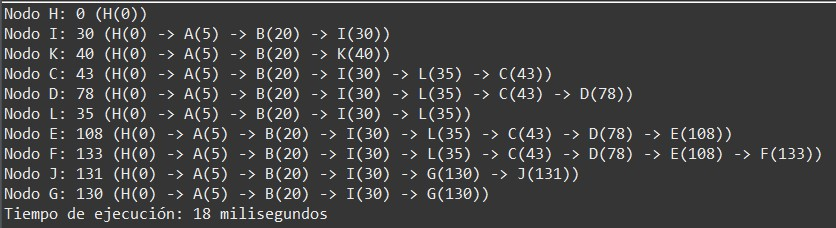
\includegraphics[width=1\linewidth]{img/Salida_codigo_secuencial_7.jpg}
	\caption{Salida por pantalla del código 1 (implementación secuencial de dijkstra)}
	\label{fig:etiqueta1}
\end{figure}

La figura muestra la salida del algoritmo, donde se presentan los pesos de los caminos óptimos desde el nodo H hasta todos los demás nodos del grafo. Para este grafo relativamente pequeño, la implementación secuencial del algoritmo de Dijkstra tarda 18 milisegundos en ejecutarse. Un análisis detallado del grafo confirma que los caminos mostrados son efectivamente los caminos óptimos.

El código 2 implementa el algoritmo de Dijkstra para encontrar el camino más corto Utilizando paralelismo para acelerar el proceso de relajación de aristas, aprovecha un ForkJoinPool y la creación de tareas paralelas como componentes clave que permite al algoritmo paralelo procesar múltiples aristas simultáneamente, potencialmente mejorando el rendimiento en grafos grandes y complejos. 

La lógica detrás de este enfoque paralelo es que la relajación de las aristas del grafo es una operación que se puede realizar de manera independiente para diferentes aristas. Por lo tanto, al ejecutar estas operaciones en paralelo, se pueden aprovechar múltiples núcleos de CPU para acelerar el proceso.

Este enfoque paralelo puede predecir resultados peores en grafos de pequeño tamaño debido al costo adicional asociado con la creación y gestión de múltiples hilos, que puede superar el beneficio del paralelismo en grafos pequeños. Sin embargo, en grafos de gran tamaño con muchas aristas, el paralelismo puede conducir a mejoras significativas en el tiempo de ejecución, ya que permite aprovechar la capacidad de procesamiento de múltiples núcleos para procesar aristas simultáneamente, lo que puede compensar el costo adicional de la paralelización.

\begin{figure}[h]
	\centering 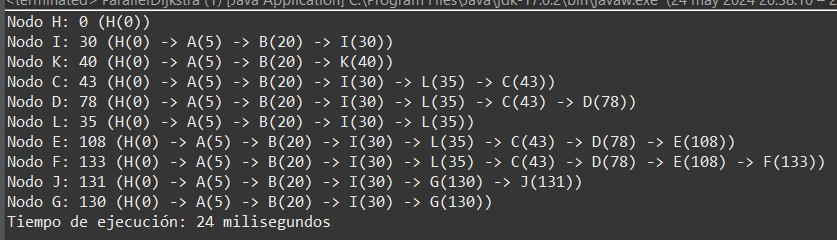
\includegraphics[width=1\linewidth]{img/Salida_codigo_paralelo_8.jpg}
	\caption{Salida por pantalla del código 2 (implementación paralela de dijkstra)}
	\label{fig:etiqueta1}
\end{figure}

En esta ocasión la salida más común es que tarde 24 milisegundos, un poco más que nuestra implementación secuencial, y aunque en ocasiones alguna compilación puede bajar hasta los 19 segundos en la mayoría de ocasiones para un grafo tan pequeño dará peores resultados que la versión secuencial. 
\begin{table}[h!]
\centering
\begin{tabular}{|p{2.5cm}|p{5cm}|p{5cm}|}
\hline
\textbf{Aspecto} & \textbf{SequentialDijkstra} & \textbf{ParallelDijkstra} \\
\hline
Ejecución & Secuencial, un solo hilo & Paralelo, múltiples hilos \\
\hline
Recorrido & Secuencialmente, una arista a la vez & Paralelamente, múltiples aristas a la vez \\
\hline
Eficiencia & Depende del número de nodos y aristas & Puede ser más eficiente en grafos grandes con muchas aristas \\
\hline
Uso de recursos & Menos uso de recursos, menor complejidad & Mayor uso de recursos debido a la creación y gestión de múltiples tareas \\
\hline
Complejidad de implementación & Relativamente simple & Más compleja debido a la necesidad de sincronización y gestión de tareas paralelas \\
\hline
\end{tabular}
\caption{Comparación entre SequentialDijkstra y ParallelDijkstra}
\label{table:comparison}
\end{table}

Los códigos 3 y 4 se han desarrollado para evaluar la escalabilidad del rendimiento de las implementaciones secuencial y paralela del algoritmo de Dijkstra. Estos códigos modifican el método main para generar nodos de forma aleatoria, incluyendo tanto letras como números. Esto permite crear grafos de diferentes tamaños, desde 24 nodos hasta un número mucho mayor, con sus correspondientes aristas.

El objetivo de esta estrategia es observar cómo la diferencia de velocidad entre las implementaciones secuencial y paralela se comporta al aumentar el tamaño del grafo. Se pretende determinar el punto a partir del cual la implementación paralela comienza a superar significativamente a la implementación secuencial en términos de rendimiento.

La gráfica 2.9 muestra el tiempo de ejecución promedio, en milisegundos, del algoritmo de Dijkstra para diferentes tamaños de grafo. Cada punto de datos representa el promedio de 10 compilaciones del algoritmo para un número específico de nodos

Si bien la gráfica 2.9 que compara el algoritmo secuencial contra el paralelo a través del aumento de nodos, esta aunque sugiere una cierta superioridad del algoritmo paralelo, es importante destacar una limitación en los resultados presentados. Durante la evaluación del rendimiento en escenarios con un número elevado de nodos, se observaron errores de manejo de valores nulos en la implementación paralela. Estos errores, resultado de la complejidad de los cálculos y la necesidad de información sobre nodos intermedios, ocasionaron la interrupción del proceso y la necesidad de recompilaciones adicionales para obtener una media precisa.

Para abordar este problema, se propone la implementación de mecanismos de concurrencia, como semáforos, que permitan gestionar el acceso a los recursos y evitar la aparición de errores. Si bien en este caso la implementación de semáforos no arrojó resultados positivos, debido a un "speedup" negativo para configuraciones con más de 20.000 nodos (posiblemente relacionado con limitaciones de memoria en Java ya que cada nodo tiene de 1 a 4 aristas), la exploración de otras técnicas de concurrencia sigue siendo una línea de investigación prometedora para optimizar el rendimiento de la implementación paralela.

\begin{figure}[h]
	\centering 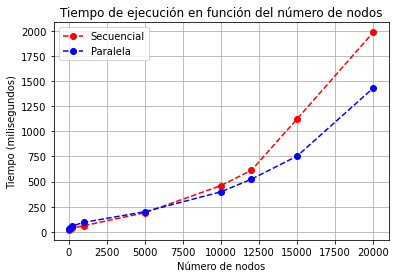
\includegraphics[width=0.75\linewidth]{img/Grafica_tiempos_9.png}
	\caption{Comparación a través del número de nodos, secuencial vs paralelo}
	\label{fig:etiqueta1}
\end{figure}


\section{Conclusiones y recomendaciones}


En este trabajo se ha evaluado la eficacia de los algoritmos de Dijkstra para la búsqueda de caminos más cortos entre todos los pares de nodos de un grafo, tanto en sus implementaciones secuencial como paralela. Los resultados obtenidos revelan un panorama alentador con algunas consideraciones importantes a tomar en cuenta que no dejan tan bien el paralelismo.

Teóricamente, se ha resaltado la naturaleza secuencial del algoritmo de Dijkstra, lo que se ha corroborado durante la implementación de su versión paralela. En este sentido, sería de gran interés extender el trabajo comparando la versión secuencial y paralela con otros algoritmos de búsqueda de caminos óptimos, como A* (Estrellas), Floyd y otros mencionados en el marco teórico.

La implementación desarrollada ha eliminado la posibilidad de errores asociados a los solapes de escrituras y lecturas que presentan muchas versiones paralelas, gracias a la concurrencia en el cálculo de los vecinos de un nodo sin tener alteraciones en una misma cuenta.

No obstante, los resultados sugieren que el algoritmo de Dijkstra no es el método más eficiente para la búsqueda de todos los caminos más cortos en un grafo en lo que paralelismo respecta. Además, su eficiencia presenta una gran variabilidad en función de las propiedades del grafo evaluado, dependiendo en gran medida del punto de inicio y la cantidad de aristas. En este sentido, se considera que un enfoque más preciso que fije un número exacto de aristas por nodo podría generar resultados más robustos y menos variables por iteración.

El capítulo concluye con un mensaje crucial: el paralelismo no es una mejora superior, sino una herramienta que ofrece una perspectiva diferente y permite alcanzar soluciones con resultados ligeramente distintos. Si bien se trata de una herramienta poderosa y valiosa, no es una solución mágica que garantice un mejor rendimiento. Este trabajo ha demostrado que su implementación puede ser compleja, especialmente en el contexto de grafos. Además, para problemas sencillos, implementar paralelismo, a pesar del esfuerzo adicional, puede generar resultados adversos. En ocasiones, dividir una tarea simple en múltiples tareas simples no se alinea con los objetivos del paralelismo. Se busca eliminar la dificultad de las tareas, no aumentarlas.


\bibliography{biblio4}

\section{Apendice (código)}

Código 1 para la construcción del grafo y aplicación de dijkstra secuencial:
\begin{lstlisting}[language=Java, style=ColorStyle]
package dijkstra_paralelo;

import java.util.*;

public class SequentialDijkstra {

    static class Graph {
        private final Map<String, Integer> nodeIndexMap;
        private final List<String> nodes;
        private final int[][] adjMatrix;

        public Graph(int maxNodes) {
            nodeIndexMap = new HashMap<>();
            nodes = new ArrayList<>();
            adjMatrix = new int[maxNodes][maxNodes];
        }

        public void addNode(String node) {
            if (!nodeIndexMap.containsKey(node)) {
                int index = nodes.size();
                nodes.add(node);
                nodeIndexMap.put(node, index);
            }
        }

        public void addEdge(String src, String dest, int weight) {
            addNode(src);
            addNode(dest);
            int srcIndex = nodeIndexMap.get(src);
            int destIndex = nodeIndexMap.get(dest);
            adjMatrix[srcIndex][destIndex] = weight;
            adjMatrix[destIndex][srcIndex] = weight; 
            // Si el grafico es no dirigido
        }

        public Result dijkstra(String startNode) {
            int V = nodes.size();
            int[] dist = new int[V];
            int[] pred = new int[V];
            Arrays.fill(dist, Integer.MAX_VALUE);
            Arrays.fill(pred, -1);
            int srcIndex = nodeIndexMap.get(startNode);
            dist[srcIndex] = 0;

            boolean[] visited = new boolean[V];
            PriorityQueue<Integer> pq = new PriorityQueue<>
            (Comparator.comparingInt(node -> dist[node]));
            pq.add(srcIndex);

            while (!pq.isEmpty()) {
                int u = pq.poll();
                if (visited[u]) continue;
                visited[u] = true;

                for (int v = 0; v < V; v++) {
                    if (!visited[v] && adjMatrix[u][v] != 0) {
                        int weight = adjMatrix[u][v];
                        if (dist[u] + weight < dist[v]) {
                            dist[v] = dist[u] + weight;
                            pred[v] = u;
                            pq.add(v);
                        }
                    }
                }
            }
            return new Result(dist, pred);
        }

        public void printResult(Result result, String startNode) {
            for (int i = 0; i < result.dist.length; i++) {
                if (result.dist[i] == Integer.MAX_VALUE) {
                    System.out.println
                    ("Nodo " + nodes.get(i) + ": Inalcanzable");
                    continue;
                }
                StringBuilder path = new StringBuilder();
                printPath(result.pred, i, path, result.dist);
                System.out.println
                ("Nodo " + nodes.get(i) + ": " + 
                result.dist[i] + " (" + path + ")");
            }
        }

        private void printPath(int[] pred, int i, 
        StringBuilder path, int[] dist) {
            if (i == -1) return;
            printPath(pred, pred[i], path, dist);
            if (path.length() > 0) {
                path.append(" -> ");
            }
            path.append(nodes.get(i)).append
            ("(").append(dist[i]).append(")");
        }

        static class Result {
            int[] dist;
            int[] pred;

            Result(int[] dist, int[] pred) {
                this.dist = dist;
                this.pred = pred;
            }
        }
    }

    public static void main(String[] args) {
        // Creacion del grafo
        Graph graph = new Graph(12); 
        // Numero maximo de nodos en el grafo

        graph.addEdge("A", "B", 15);
        graph.addEdge("A", "H", 5);
        graph.addEdge("B", "I", 10);
        graph.addEdge("B", "K", 20);
        graph.addEdge("C", "D", 35);
        graph.addEdge("C", "L", 8);
        graph.addEdge("D", "E", 30);
        graph.addEdge("D", "I", 50);
        graph.addEdge("E", "F", 25);
        graph.addEdge("E", "J", 35);
        graph.addEdge("F", "K", 200);
        graph.addEdge("G", "I", 100);
        graph.addEdge("G", "J", 1);
        graph.addEdge("H", "L", 9999);
        graph.addEdge("I", "L", 5);

        // Obtener el tiempo de inicio
	    long inicio = System.nanoTime();
        Graph.Result result = graph.dijkstra("H");
        System.out.println("Distancias desde el nodo H:");
        graph.printResult(result, "H");
        
     // Obtener el tiempo de finalizacion
	    long fin = System.nanoTime();
	      
	    // Calcular la duracion de la ejecucion
	    long t = (fin - inicio) / 1_000_000; 
	    // Convertir de nanosegundos a milisegundos
	      
	    System.out.println
     ("Tiempo de ejecucion: " + t + " milisegundos");
    }
}

	\end{lstlisting}

Código 2 para la creación de un grafo y llamada del algoritmo de dijkstra versión con concurrencia:
\begin{lstlisting}[language=Java, style=ColorStyle]
package dijkstra_paralelo;

import java.util.concurrent.*;
import java.util.*;

public class ParallelDijkstra {

    static class Graph {
        private final Map<String, Integer> nodeIndexMap;
        private final List<String> nodes;
        private final int[][] adjMatrix;

        public Graph(int maxNodes) {
            nodeIndexMap = new HashMap<>();
            nodes = new ArrayList<>();
            adjMatrix = new int[maxNodes][maxNodes];
        }

        public void addNode(String node) {
            if (!nodeIndexMap.containsKey(node)) {
                int index = nodes.size();
                nodes.add(node);
                nodeIndexMap.put(node, index);
            }
        }

        public void addEdge(String src, String dest, int weight) {
            addNode(src);
            addNode(dest);
            int srcIndex = nodeIndexMap.get(src);
            int destIndex = nodeIndexMap.get(dest);
            adjMatrix[srcIndex][destIndex] = weight;
            adjMatrix[destIndex][srcIndex] = weight; 
            // Si el grafico es no dirigido
        }

        public Result parallelDijkstra(String startNode) throws
        InterruptedException, ExecutionException {
            int V = nodes.size();
            int[] dist = new int[V];
            int[] pred = new int[V];
            Arrays.fill(dist, Integer.MAX_VALUE);
            Arrays.fill(pred, -1);
            int srcIndex = nodeIndexMap.get(startNode);
            dist[srcIndex] = 0;

            boolean[] visited = new boolean[V];
            PriorityQueue<Integer> pq = new 
            PriorityQueue<>
            (Comparator.comparingInt(node -> dist[node]));
            pq.add(srcIndex);

            ForkJoinPool forkJoinPool = new ForkJoinPool();
            while (!pq.isEmpty()) {
                int u = pq.poll();
                if (visited[u]) continue;
                visited[u] = true;

                List<Callable<Void>> tasks = new ArrayList<>();
                for (int v = 0; v < V; v++) {
                    if (!visited[v] && adjMatrix[u][v] != 0) {
                        final int node = 
                        v;
                        //Definir node como final
                        int weight = adjMatrix[u][node];
                        tasks.add(() -> {
                            if (dist[u] + weight < dist[node]) {
                                dist[node] = dist[u] + weight;
                                pred[node] = u;
                                pq.add(node);
                            }
                            return null;
                        });
                    }
                }
                forkJoinPool.invokeAll(tasks);
            }
            forkJoinPool.shutdown();
            return new Result(dist, pred);
        }

        public void printResult(Result result, String startNode) {
            for (int i = 0; i < result.dist.length; i++) {
                if (result.dist[i] == Integer.MAX_VALUE) {
                    System.out.println
                    ("Nodo " + nodes.get(i) + ": Inalcanzable");
                    continue;
                }
                StringBuilder path = new StringBuilder();
                printPath(result.pred, i, path, result.dist);
                System.out.println
                ("Nodo " + nodes.get(i) + ": " +
                result.dist[i] + " (" + path + ")");
            }
        }

        private void printPath
        (int[] pred, int i, StringBuilder path, int[] dist) {
            if (i == -1) return;
            printPath(pred, pred[i], path, dist);
            if (path.length() > 0) {
                path.append(" -> ");
            }
            path.append(nodes.get(i)).append
            ("(").append(dist[i]).append(")");
        }

        static class Result {
            int[] dist;
            int[] pred;

            Result(int[] dist, int[] pred) {
                this.dist = dist;
                this.pred = pred;
            }
        }
    }

    public static void main(String[] args) 
    throws InterruptedException, ExecutionException {
        // Creacion del grafo
        Graph graph = new Graph(12); 
        // Numero maximo de nodos en el grafo

        graph.addEdge("A", "B", 15);
        graph.addEdge("A", "H", 5);
        graph.addEdge("B", "I", 10);
        graph.addEdge("B", "K", 20);
        graph.addEdge("C", "D", 35);
        graph.addEdge("C", "L", 8);
        graph.addEdge("D", "E", 30);
        graph.addEdge("D", "I", 50);
        graph.addEdge("E", "F", 25);
        graph.addEdge("E", "J", 35);
        graph.addEdge("F", "K", 200);
        graph.addEdge("G", "I", 100);
        graph.addEdge("G", "J", 1);
        graph.addEdge("H", "L", 9999);
        graph.addEdge("I", "L", 5);

        // Obtener el tiempo de inicio
	    long inicio = System.nanoTime();
	    		  
        Graph.Result result = graph.parallelDijkstra("H");
        System.out.println("Distancias desde el nodo H:");
        graph.printResult(result, "H");
        
        // Obtener el tiempo de finalizacion
	    long fin = System.nanoTime();
	      
	    // Calcular la duracion de la ejecucion
	    long t = (fin - inicio) / 1_000_000; 
	    // Convertir de nanosegundos a milisegundos
	      
	    System.out.println
     ("Tiempo de ejecucion: " + t + " milisegundos");
    }
}

\end{lstlisting}
	
Código 3 método que crea grafos con N + 64 nodos y se aplica  el dijkstra secuencial
\begin{lstlisting}[language=Java, style=ColorStyle]
package dijkstra_paralelo;

import java.util.*;
import java.util.concurrent.ExecutionException;

public class SequentialDijkstraWithLargeGraph {

    public static void main(String[] args) {
        Scanner scanner = new Scanner(System.in);

        System.out.print
        ("Ingrese el numero maximo de nodos en el grafo: ");
        int n = scanner.nextInt();

        SequentialDijkstra.grafo graph = new
        SequentialDijkstra.grafo(n + 64); 
        // Numero maximo de nodos en el grafo

        // Generar aristas con valores aleatorios entre 1 y 100
        Random random = new Random();
        for (char c1 = 'A'; c1 <= 'Z'; c1++) {
            for (char c2 = 'A'; c2 <= 'Z'; c2++) {
                if (c1 != c2) { // Evitar lazos
                    int weight = random.nextInt(100) + 1; 
                    // Valor aleatorio entre 1 y 100
                    graph.addEdge(String.valueOf(c1),
                    String.valueOf(c2), weight);
                }
            }
        }
        for (char c1 = 'a'; c1 <= 'z'; c1++) {
            for (char c2 = 'A'; c2 <= 'Z'; c2++) {
                if (c1 != c2) { // Evitar lazos
                    int weight = random.nextInt(100) + 1; 
                    // Valor aleatorio entre 1 y 100
                    graph.addEdge(String.valueOf(c1), 
                    String.valueOf(c2), weight);
                }
            }
        }

        // Agregar 120 aristas mas
        for (int i = 0; i < 120; i++) {
            char c1 = (char) ('A' + random.nextInt(26));
            char c2 = (char) ('A' + random.nextInt(26));
            int weight = random.nextInt(100) + 1;
            // Valor aleatorio entre 1 y 100
            graph.addEdge(String.valueOf(c1), 
            String.valueOf(c2), weight);
        }

        // Agregar nodos con nombres del 1 al n
        for (int i = 1; i <= n; i++) {
            graph.addEdge(String.valueOf(i), 
            String.valueOf(i), 0); // Agregar nodo con peso 0
        }

        // Agregar n aristas adicionales entre nodos
        for (int i = 0; i < n; i++) {
            int node1 = random.nextInt(n) + 1; 
            // Nodo aleatorio del 1 al n
            int node2 = random.nextInt(n) + 1; 
            // Nodo aleatorio del 1 al n
            int weight = random.nextInt(200) + 1; 
            // Valor aleatorio entre 1 y 200
            graph.addEdge(String.valueOf(node1), 
            String.valueOf(node2), weight);
        }

        // Agregar aristas que conecten nodos 
        //numericos con nodos de letras minusculas
        for (int i = 1; i <= n; i++) {
            char letter = (char) ('a' + random.nextInt(26)); 
            // Letra minuscula aleatoria
            int weight = random.nextInt(200) 
            + 1; // Valor aleatorio entre 1 y 200
            graph.addEdge(String.valueOf(i),
            String.valueOf(letter), weight);
        }

        // Obtener el tiempo de inicio
        long inicio = System.nanoTime();
        SequentialDijkstra.grafo.Result 
        result = graph.dijkstra("H");
        System.out.println("Distancias desde el nodo H:");
        graph.printResult(result, "H");

        // Obtener el tiempo de finalizacion
        long fin = System.nanoTime();

        // Calcular la duracion de la ejecucion
        long t = (fin - inicio) / 1_000_000; 
        // Convertir de nanosegundos a milisegundos

        System.out.println
        ("Tiempo de ejecucion: " + t + " milisegundos");

        scanner.close();
    }
}


\end{lstlisting}

Código 4 método que crea grafos con N + 64 nodos y se aplica  el dijkstra paralelo
\begin{lstlisting}[language=Java, style=ColorStyle]
package dijkstra_paralelo;

import java.util.*;
import java.util.concurrent.ExecutionException;

public class ParallelDijkstraWithLargeGraph {

    public static void main(String[] args) {
        Scanner scanner = new Scanner(System.in);

        System.out.print
        ("Ingrese el numero maximo de nodos en el grafo: ");
        int n = scanner.nextInt();

        ParallelDijkstra.Graph graph = new 
        ParallelDijkstra.Graph(n + 64); 

// Grafo con letras desde A hasta Z (mayusculas y minusculas) 
//y numeros del 1 al n

        // Agregar aristas con valores aleatorios entre 1 y 100
        Random random = new Random();
        for (char c1 = 'A'; c1 <= 'Z'; c1++) {
            for (char c2 = 'A'; c2 <= 'Z'; c2++) {
                if (c1 != c2) { // Evitar lazos
                    int weight = random.nextInt(100) + 1; 
// Valor aleatorio entre 1 y 100
                    graph.addEdge(String.valueOf(c1),
                    String.valueOf(c2), weight);
                }
            }
        }
        for (char c1 = 'a'; c1 <= 'z'; c1++) {
            for (char c2 = 'A'; c2 <= 'Z'; c2++) {
                if (c1 != c2) { // Evitar lazos
                    int weight = random.nextInt(100) + 1; 
                    // Valor aleatorio entre 1 y 100
                    graph.addEdge(String.valueOf(c1),
                    String.valueOf(c2), weight);
                }
            }
        }

        // Agregar 120 aristas mas
        for (int i = 0; i < 120; i++) {
            char c1 = (char) ('A' + random.nextInt(26));
            char c2 = (char) ('A' + random.nextInt(26));
            int weight = random.nextInt(100) + 1; 
            // Valor aleatorio entre 1 y 100
            graph.addEdge(String.valueOf(c1), 
            String.valueOf(c2), weight);
        }
        
        // Agregar nodos con nombres del 1 al n
        for (int i = 1; i <= n; i++) {
            graph.addEdge(String.valueOf(i), 
            String.valueOf(i), 0); 
            // Agregar nodo con peso 0
        }
        // Agregar n aristas adicionales entre nodos
        for (int i = 0; i < n; i++) {
            int node1 = random.nextInt(n) + 1; 
            // Nodo aleatorio del 1 al n
            int node2 = random.nextInt(n) + 1; 
            // Nodo aleatorio del 1 al n
            int weight = random.nextInt(200) + 1; 
            // Valor aleatorio entre 1 y 200
            graph.addEdge(String.valueOf(node1), 
            String.valueOf(node2), weight);
        }

        // Agregar aristas que conecten nodos 
        //numericos con nodos de letras minusculas
        for (int i = 1; i <= n; i++) {
            char letter = (char) ('a' + random.nextInt(26)); 
            // Letra minuscula aleatoria
            int weight = random.nextInt(200) + 1; 
            // Valor aleatorio entre 1 y 200
            graph.addEdge(String.valueOf(i), 
            String.valueOf(letter), weight);
        }
        // Obtener el tiempo de inicio
        long inicio = System.nanoTime();
        ParallelDijkstra.Graph.Result result = null;
        try {
            result = graph.parallelDijkstra("H");
        } catch (InterruptedException e) {
            e.printStackTrace();
        } catch (ExecutionException e) {
            e.printStackTrace();
        }
        System.out.println("Distancias desde el nodo H:");
        graph.printResult(result, "H");

        // Obtener el tiempo de finalizacion
        long fin = System.nanoTime();

        // Calcular la duracion de la ejecucion
        long t = (fin - inicio) / 1_000_000;
        // Convertir de nanosegundos a milisegundos

        System.out.println
        ("Tiempo de ejecucion: " + t + " milisegundos");

        scanner.close();
    }
}

\end{lstlisting}